\documentclass{standalone}
\usepackage{tikz}
\usetikzlibrary{arrows,calc}
\begin{document}

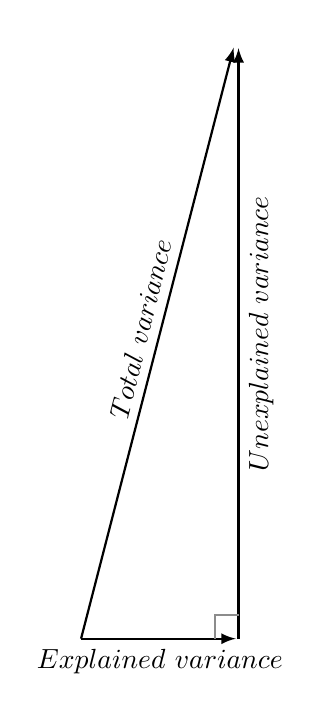
\begin{tikzpicture}[
  to/.style={->,>=latex,shorten
    >=7 pt,thick,font=\sffamily\normalsize}, 
 right angle quadrant/.code={
        \pgfmathsetmacro\quadranta{{1,1,-1,-1}[#1-1]}     % Arrays for selecting quadrant
        \pgfmathsetmacro\quadrantb{{1,-1,-1,1}[#1-1]}},
    right angle quadrant=1, % Make sure it is set, even if not called explicitly
    right angle length/.code={\def\rightanglelength{#1}},   % Length of symbol
    right angle length=2ex, % Make sure it is set...
  right angle symbol/.style n args={3}{
        insert path={
            let \p0 = ($(#1)!(#3)!(#2)$) in     % Intersection
                let \p1 = ($(\p0)!\quadranta*\rightanglelength!(#3)$), % Point on base line
                \p2 = ($(\p0)!\quadrantb*\rightanglelength!(#2)$) in % Point on perpendicular line
                let \p3 = ($(\p1)+(\p2)-(\p0)$) in  % Corner point of symbol
            (\p1) -- (\p3) -- (\p2)
        }
    }
]

 \coordinate (a) at (0,0);
 \coordinate (b) at (2,0);
 \coordinate (c) at (2,7.746);

 \draw[to, shorten >=1 pt,] (a) -- (b) node[midway,below, rotate=0] {$Explained\,\, variance$};
 \draw[to] (a) -- (c) node[midway,above, rotate=76] {$Total\,\, variance$};
 \draw[to] (b) -- (c) node[midway,below, rotate=90] {$Unexplained\,\,
   variance$};
\draw [gray!90,thick,right angle symbol={c}{b}{a}];
\end{tikzpicture}
\end{document}

 \coordinate (b) at (7.746,0);
 \coordinate (c) at (7.746,2);
